%!TEX root = ../thesis.tex

\chapter{Implementation}
\label{ch:implementation}

Text text

\section{Existing implementation}

As we have already mentioned, an implementation has already been attempted for this project.
Before we can begin with a new one, we first have to decide which parts of it we want to use, and which to discard.
These parts are summarized in this section.

\subsection{SCM Expansion}
\label{sec:scm_expansion}

The SCM package has been expanded for GitHub to support the following functions:

\begin{itemize}
    \item CreateIssue   - creates an issue on a repository.
    \item EditRepoIssue - edits an issue on a repository.
    \item GetRepoIssue  - retrieves an issue based on issue number and repository.
    \item GetRepoIssues - retrieves all issues from a repository.
\end{itemize}

CreateIssue and EditRepoIssue would prove useful, and are used with only minor adjustments to them.
The two other functions, centered around retrieving issues were not needed, but still used in earlier parts of the project when testing.

\subsection{Logic}

A lot of existing code was intended to handle the logic around managing tasks. 
In short, this code was meant to do determine when to create, edit or delete issues on GitHub.
The code did however not accomplish this in a functional manner.
This lead to the dilemma of whether to continue developing this faulty code, or simply start anew.
In the end, we decided that any attempt to fix the existing logic code would be more time consuming and confusing than simply starting fresh.

\subsection{Parsing Tasks}
\label{sec:parsing_tasks}

When a teacher pushes assignments to the \textit{tests} repository, QuickFeed will run the function UpdateFromTestsRepo.
In short, this function creates a local copy of the folder structure found in \textit{tests}, and uses it to create or update the data-record of every assignment.
Added as a part of this process, was code to also fetch all task markdown files in the repository, and use their contents to create a task data object.

To support this, all \textit{task-*.md} files are expected to conform to a standard format.
The first line should start with the character sequence "\# <task title>", followed by by two new line characters.
Any following text there after will be treated as the task body or description.

Using this format, the function newTask creates a task data object from any task file.

\lstinputlisting[caption={Function that creates a task object from markdown content}, language=Golang, firstline=25, lastline=40]{code/tasks.go}

Going forward, the general approach to parsing and creating tasks is left as it is, with only minor changes to the existing code.

\section{Managing Tasks and Issues}

Having looked at what existing code we decided to keep, we continue by exploring the part of the project that was implemented first; how to manage tasks and issues.

Moving forward in this chapter, we make the following distinction between found tasks/assignments, and existing tasks/assignments.
Found tasks and assignments are data objects created from the contents found within the \textit{tests} repository.
Existing tasks and assignments are data-objects based on data records that we retrieve from the database.

\subsection{Overview}

This section gives an overview of the features QuickFeed will support through this implementation.

Teachers can now create \textit{task-*.md} files inside individual assignments in \textit{tests}, as illustrated below.

\begin{figure}[ht]
    \centering
    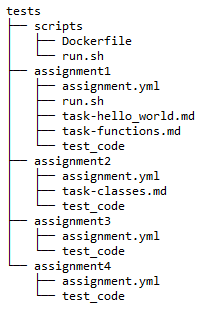
\includegraphics[scale=0.8]{photos/tests-repository-structure-tasks.PNG}
    \caption{Example of a tests repository with tasks}
    \label{fig:tests-repository-structure-tasks}
\end{figure}

When they are pushed to GitHub, an issue is created on every group repository to represent them.
When teachers changes a task, either by editing it or deleting it, these changes are reflected on their associated issues.
I.e. every issue is in sync with the task that created it.

\subsection{Data Structures}

Two new messages are defined in the ag.proto file: \textbf{Task} and \textbf{Issue}.
These are used to generate the data structures that we use throughout the rest of the project.

\textbf{Task} is defined as follows:

\lstinputlisting[caption={Task message}, firstline=185, lastline=193]{code/ag.proto}

Every task is associated with one assignment via the \textit{assignmentID} field.

For an assignment, \textit{order} is a number used to determine the order in which it is represented in a course.
It is set by a teacher in the assignment \textit{assignment.yml} file, which is described in section \ref{sec:quickfeed-repository-structure}.
When we create a new task, keeping track of the corresponding assignment order is useful.
It allows us to associate tasks and assignments without explicitly knowing the assignment ID, so long as our scope is limited to just a single course.
A feature that will prove necessary.

The \textit{name} field is used to associate tasks found in \textit{tests}, with the ones stored in the database.
If a task file with the name task-hello\_world.md is found within assignment1, then its corresponding name will be assignment1/hello\_world.
This name is set when the task itself is parsed, as described in section \ref{sec:parsing_tasks}.

\textbf{Issue} is defined as follows:

\lstinputlisting[caption={Issue message}, firstline=195, lastline=200]{code/ag.proto}

We see that every issue holds an association to the task that was used to create it, as well as the repository it was created on.

The \textit{issueNumber} field represents the issue number GitHub will assign the issue on its creation.

As it will become important in the next section, we will also mention that a modification was made to the existing message \textbf{Assignment}.

\lstinputlisting[caption={Assignment message}, firstline=168, lastline=183]{code/ag.proto}

On line 14 on the above code we see that the message has repeated tasks.
When we compile it, the resulting data structure can hold a list of tasks.

\subsection{Main Logic}

As mentioned in section \ref{sec:parsing_tasks}, UpdateFromTestsRepo is run when someone pushes to the \textit{tests} repository.
Since tasks and issues need to be synchronized every time this happens, all logic for doing so will happen here.

More specifically, we create the function handleTasks that manages all logic relating to tasks.
It is supplied with every found assignment, and their respective found tasks, as an argument.
The function itself is run at the end of UpdateFromTestsRepo.

\lstinputlisting[caption={The function handleTasks, responsible for all task related logic}, 
                language=Golang, label={code:handleTasks}, firstline=64, lastline=95]{code/tasks.go}

The logic contained in this function will be explained in the following sections.

\subsection{Synchronizing Tasks}

When teachers create, edit, and delete tasks, we must make sure that the same happens in QuickFeed's internal database.
To accomplish this, we create the database method SynchronizeAssignmentTasks.
This method is run at the start of handleTasks, and can be summarized in the following chart.

\begin{figure}[ht]
    \centering
    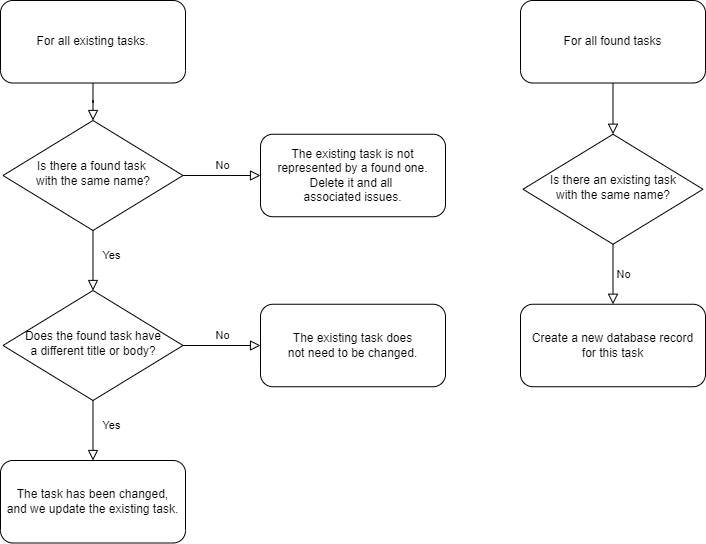
\includegraphics[width=\textwidth]{photos/synchronize-tasks-flow-chart.png}
    \caption{Flow chart describing how tasks are synchronized}
    \label{fig:synchronize-tasks-flow-chart}
\end{figure}

To support this logic, SynchronizeAssignmentTasks utilizes Go's built in maps to map tasks by both assignment order and name.
Given that we are limited in scope to a single course, we can use this mapping to associate every existing task to their found counterpart.

\lstinputlisting[caption={Logic performed in SynchronizeAssignmentTasks}, 
                language=Golang, label={code:SynchronizeAssignmentTasks}, firstline=41, lastline=76]{code/gormdb_tasks.go}

SynchronizeAssignmentTasks also returns the tasks it has created or updated, which will be important when synchronizing issues.

\subsection{Synchronizing Issues}

When we synchronize issues we must make sure to synchronize not only the issues stored in the database, but also the GitHub issues themselves.

As mentioned, SynchronizeAssignmentTasks already determines which tasks have been created, updated or deleted.
In fact, when it detects that a task has been deleted, it deletes not only the task but all associated issue records, as seen on line 11 in code \ref{code:SynchronizeAssignmentTasks}.
Issue data records also never need to be updated, since they carry no other information than an issue number, which always remains static.
The only remaining database related synchronization for issues is therefore creating them.

To delete issues, we wanted to expand on this API to give it that capacity.
It turns out however, that GitHub's REST API does not support deleting issues.
An alternative could be to use GraphQL, a query language for API's, but instead we went for a simpler solution.

Instead of deleting issues, they are closed, and their title and body are inserted with a statement indicating that the associated task has been deleted.

The entire process of synchronizing issues happens on line 16 to 31 in handleTasks \ref{code:handleTasks}.
In short, we use the created and updated tasks returned by SynchronizeAssignmentTasks, as arguments in createIssues and updateIssues respectively.
These functions use the SCM functions described in section \ref{sec:scm_expansion}.
Then, by looping through every course group repository we create and update GitHub issues accordingly.
createIssues also returns a list of all the issues it created.
These are used at the end of the process to create issue database records.

It is worth mentioning that we did not discuss how we delete GitHub issues in the above process.
To delete issues, we wanted to expand on the SCM API to give it that capacity.
It turns out however, that GitHub's REST API does not support deleting issues.
An alternative could be to use GraphQL, a query language for API's, but instead we went for a simpler solution.
Instead of deleting issues, they are closed, and their title and body are inserted with a statement indicating that the associated task has been deleted.

% In pr chapter, need to discuss if QF should create PR's or students